
%% bare_conf.tex
%% V1.4
%% 2012/12/27
%% by Michael Shell
%% See:
%% http://www.michaelshell.org/
%% for current contact information.
%%
%% This is a skeleton file demonstrating the use of IEEEtran.cls
%% (requires IEEEtran.cls version 1.8 or later) with an IEEE conference paper.
%%
%% Support sites:
%% http://www.michaelshell.org/tex/ieeetran/
%% http://www.ctan.org/tex-archive/macros/latex/contrib/IEEEtran/
%% and
%% http://www.ieee.org/

%%*************************************************************************
%% Legal Notice:
%% This code is offered as-is without any warranty either expressed or
%% implied; without even the implied warranty of MERCHANTABILITY or
%% FITNESS FOR A PARTICULAR PURPOSE! 
%% User assumes all risk.
%% In no event shall IEEE or any contributor to this code be liable for
%% any damages or losses, including, but not limited to, incidental,
%% consequential, or any other damages, resulting from the use or misuse
%% of any information contained here.
%%
%% All comments are the opinions of their respective authors and are not
%% necessarily endorsed by the IEEE.
%%
%% This work is distributed under the LaTeX Project Public License (LPPL)
%% ( http://www.latex-project.org/ ) version 1.3, and may be freely used,
%% distributed and modified. A copy of the LPPL, version 1.3, is included
%% in the base LaTeX documentation of all distributions of LaTeX released
%% 2003/12/01 or later.
%% Retain all contribution notices and credits.
%% ** Modified files should be clearly indicated as such, including  **
%% ** renaming them and changing author support contact information. **
%%
%% File list of work: IEEEtran.cls, IEEEtran_HOWTO.pdf, bare_adv.tex,
%%                    bare_conf.tex, bare_jrnl.tex, bare_jrnl_compsoc.tex,
%%                    bare_jrnl_transmag.tex
%%*************************************************************************

\documentclass[conference]{IEEEtran}

\usepackage{graphicx}
\graphicspath{{images/}}

\usepackage{url}
% url.sty was written by Donald Arseneau. It provides better support for
% handling and breaking URLs. url.sty is already installed on most LaTeX
% systems. The latest version and documentation can be obtained at:
% http://www.ctan.org/tex-archive/macros/latex/contrib/url/
% Basically, \url{my_url_here}.

% correct bad hyphenation here
\hyphenation{op-tical net-works semi-conduc-tor}

\begin{document}

\title{UGAN: Underwater Image Restoration using Generative Adversarial Networks}

\author{\IEEEauthorblockN{Cameron Fabbri}
\IEEEauthorblockA{Information Directorate\\
Air Force Research Laboratory \\
Rome, NY, USA.\\
cameron.fabbri@us.af.mil}
\and
\IEEEauthorblockN{Md Jahidul Muslim}
\IEEEauthorblockA{UMN\\}
\and
\IEEEauthorblockN{Junaed Sattar}
\IEEEauthorblockA{UMN\\
}}

% for over three affiliations, or if they all won't fit within the width
% of the page, use this alternative format:
% 
%\author{\IEEEauthorblockN{Michael Shell\IEEEauthorrefmark{1},
%Homer Simpson\IEEEauthorrefmark{2},
%James Kirk\IEEEauthorrefmark{3}, 
%Montgomery Scott\IEEEauthorrefmark{3} and
%Eldon Tyrell\IEEEauthorrefmark{4}}
%\IEEEauthorblockA{\IEEEauthorrefmark{1}School of Electrical and Computer Engineering\\
%Georgia Institute of Technology,
%Atlanta, Georgia 30332--0250\\ Email: see http://www.michaelshell.org/contact.html}
%\IEEEauthorblockA{\IEEEauthorrefmark{2}Twentieth Century Fox, Springfield, USA\\
%Email: homer@thesimpsons.com}
%\IEEEauthorblockA{\IEEEauthorrefmark{3}Starfleet Academy, San Francisco, California 96678-2391\\
%Telephone: (800) 555--1212, Fax: (888) 555--1212}
%\IEEEauthorblockA{\IEEEauthorrefmark{4}Tyrell Inc., 123 Replicant Street, Los Angeles, California 90210--4321}}

% make the title area
\maketitle

% As a general rule, do not put math, special symbols or citations
% in the abstract
\begin{abstract}
Autonomous underwater robots often rely on visual input for decision making due to its non-intrusive and passive nature
. However, due to many factors such as light refraction, particles in the water, and color distortion, images are often times very noisy. This paper propose a method using Generative Adversarial Networks (GANs) to denoise underwater images, and show that these images provide both increased accuracy
for an underwater tracking algorithm, as well as a more visually appealing image. Furthermore, we show how recently
proposed methods are able to generate a dataset for the purpose of underwater image reconstruction.
\end{abstract}

\IEEEpeerreviewmaketitle

\section{Introduction}
Vision is a commonly used sensor in autonomous underwater robots due to its non-intrusive, passive, and energy
effecient nature. The monitoring of coral reefs \cite{shkurti2012multi}, deep ocean exploration
\cite{whitcomb2000advances}, and mapping of the seabed are all tasks suitable for autonomous robots because they
provide safety by taking the risk instead of a human. Despite the advantages vision provides, many underwater
environments can be quite noisy due to light refraction and particles present in the water. Because red wavelengths are
quickly absorbed by water, images tend to have a green or blue hue to them. As you go deeper, this worsens as more
and more red wavelengths are being absorbed. This extremely non-linear distortion has many factors such as the amount
of light present (overcast vs sunny or depth), particles in the water, time of day, and the camera being used. This may
cause difficulty in tasks such as segmentation, tracking, or classification due to their indirect or direct use of
color.

As color and illumination begin to change with the depth, vision based algorithms must be very generalizable in order
to work within the depth ranges a robot may operate in. Because of the high cost and difficulty of acquiring a
variety of underwater data, as well as the high amount of noise introduced, many algorithms may perform poorly in
these different domains. Figure 1 shows the high variability that may occur in underwater vision. A step towards a
solution to this
issue is to be able to restore the images such that they appear to be above water, i.e., with colors corrected and
particles removed. By performing a many to one mapping of these domains from underwater to not underwater (what the
image would look like in the air), algorithms that have

\begin{figure}[!htb]
   \begin{center}$
      \begin{array}{cccc}
         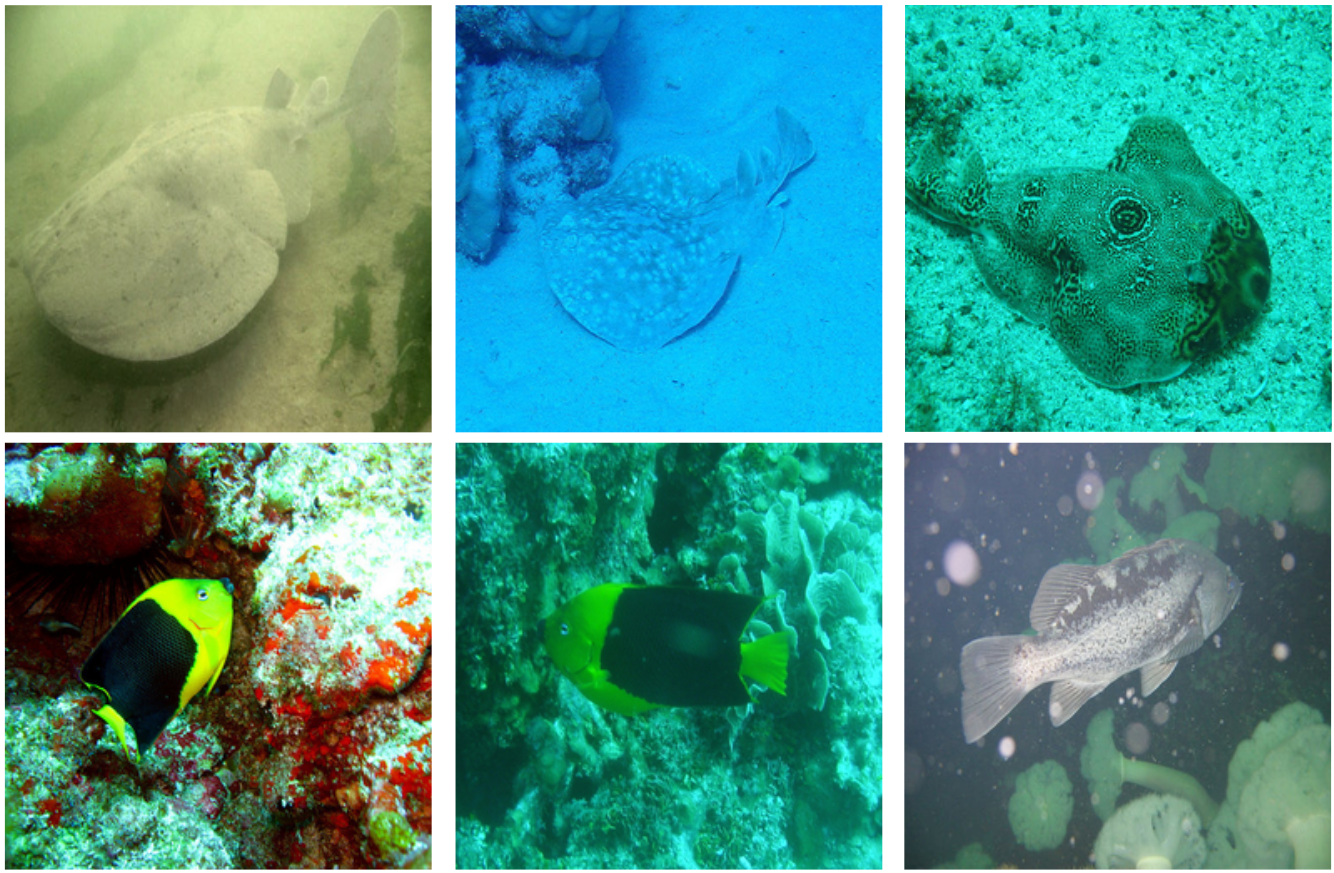
\includegraphics[width=3in]{figure1}
      \end{array}$
   \end{center}
   \caption{Underwater images showing the vast divesity of noise that can occur, including
   different hues of green and blue, as well as particles in the water.}
\end{figure}

\noindent difficulty performing across multiple forms of noise may be able to focus only one clean domain.

Deep neural networks have been shown to be powerful non-linear function approximators, especially in the field of
vision. Often times, these networks recquire large amounts of data, either labeled or paired with ground truth.
For the problem of automatically colorizing grayscale images, paired training data is essentially free due to the
fact that any color image can be converted to black and white. However, underwater images distorted by either color
or some other visual effect lack ground truth. We use the recently proposed CycleGAN \cite{zhu2017unpaired}, which
learns to translate an image from domain $X$ to domain $Y$, as a way to generate a paired dataset. By letting $X$ be
a set of undistorted underwater images, and $Y$ be a set of distorted underwater images, we can generate an image
that appears to be underwater while retaining ground truth.

\section{Related Work}

While there have been many very successful recent approaches towards colorization
\cite{zhang2016colorful,iizuka2016let}, all are focused on the task of grayscale to color. Color correction and image
restoration for the underwater domain has been less explored. The work of \cite{torres2005color} used an energy
minimization formulation using a Markov Random Field. 


\section{Method}
Recent work in generative models, specifically Generative Adversarial
Networks (GANs), have shown great success in areas such as inpainting \cite{pathak2016context}, style transfer
\cite{Gatys_2016_CVPR}, and image-to-image translation \cite{isola2016image,zhu2017unpaired}. This is highly due to
their ability to provide a more meaningful loss than simply the Euclidean distance, which has been shown to produce
blurry results. 


\subsection{Generative Adversarial Networks}



\subsection{Objective}



\subsection{Network Architectures}


\subsubsection{Training details}

L1 weight 100, batch size 32, wgan loss, learning rate 1e-4, IG weight 1.0 and 0.0, 100 epochs


\subsubsection{Generator}



\subsubsection{Discriminator}



\section{Conclusion}



\section*{Acknowledgment}

%
%\begin{thebibliography}{1}
%\bibitem{hires}{Johnson‐Roberson, Matthew, et al. "High‐Resolution Underwater Robotic Vision‐Based Mapping and Three‐Dimensional Reconstruction for Archaeology." Journal of Field Robotics 34.4 (2017): 625-643.}
%
%\bibitem{col1}{Zhang, Richard, Phillip Isola, and Alexei A. Efros. "Colorful image colorization." European Conference on Computer Vision. Springer International Publishing, 2016.}

%\bibitem{col2}{Cheng, Zezhou, Qingxiong Yang, and Bin Sheng. "Deep colorization." Proceedings of the IEEE International Conference on Computer Vision. 2015.}

%\bibitem{col3}{Iizuka, Satoshi, Edgar Simo-Serra, and Hiroshi Ishikawa. "Let there be color!: joint end-to-end learning of global and local image priors for automatic image colorization with simultaneous classification." ACM Transactions on Graphics (TOG) 35.4 (2016): 110.}

%\bibitem{pix2pix}{Isola, Phillip, et al. "Image-to-image translation with conditional adversarial networks." arXiv preprint arXiv:1611.07004 (2016).}

%\bibitem{watergan}{Li, Jie, et al. "WaterGAN: Unsupervised Generative Network to Enable Real-time Color Correction of Monocular Underwater Images." arXiv preprint arXiv:1702.07392 (2017).}

%\end{thebibliography}

%\bibliography{/home/fabbric/Research/colorCorrection/files/paper/cambibs}
\bibliography{cambibs}
\bibliographystyle{ieeetr}

% that's all folks
\end{document}


